\documentclass[11pt]{article}

% Template-agnostic preamble (matches the WANDERING-arc papers).
\usepackage[margin=1in]{geometry}
\usepackage[utf8]{inputenc}
\usepackage[T1]{fontenc}
\usepackage{hyperref}
\hypersetup{colorlinks=true, linkcolor=blue, citecolor=blue, urlcolor=blue,
  pdftitle={The Lever Is Late: Causal Control of Long-Horizon Agent Termination Lives in a Task-Matched, Late Action-Commitment Block},
  pdfauthor={Caio Vicentino}}
\emergencystretch=3em
\sloppy
\hyphenpenalty=2000
\exhyphenpenalty=0
\hbadness=10000
\usepackage{booktabs}
\usepackage{amsfonts}
\usepackage{amsmath}
\usepackage{amssymb}
\usepackage{xcolor}
\usepackage{array}
\usepackage{graphicx}

\title{The Lever Is Late: \\
Causal Control of Long-Horizon Agent Termination Lives in a \\
Task-Matched, Late Action-Commitment Block \\[2pt]
\large The first positive of the WANDERING arc}

\author{%
  Caio Vicentino \\
  OpenInterpretability \\
  Fortaleza, Brazil \\
  ORCID: 0009-0003-4331-6259 \\
  \texttt{caio@openinterp.org}%
}
\date{June 2026}

\begin{document}
\maketitle

\begin{abstract}
A long-horizon coding agent fails in a distinctive way we call \textbf{WANDERING}: it keeps acting --- reading, editing, running commands --- but never emits the \texttt{finish} action, exhausting its turn budget. A five-part study established a stark detection--control asymmetry around this failure: the agent's ``the task is done'' verdict is linearly decodable (AUROC $0.81$--$0.91$) yet causally inert --- no residual-stream injection rescues termination, and clamping the \emph{exact, named} SAE ``done'' feature moves the probability of finishing by $-0.001$. After five places where control is \emph{not}, this paper asks where it \emph{is}. On 99 SWE-bench Pro trajectories (Qwen3.6-27B), reconstructed faithfully at the decision point and gated for behavioral fidelity (P(\texttt{finish}): \textsc{success} $0.59 \gg$ \textsc{wandering} $0.07 \gg$ \textsc{locked} $0.005$), a layer-resolved logit-lens shows the finish decision is invisible through layer~31 and emerges only in the last $\sim$12 layers (L51--L63), $\sim$30 layers \emph{downstream} of the mid-layer verdict (L23). Activation patching confirms the asymmetry causally: injecting the \textsc{success} late-block state into \textsc{wandering} raises P(\texttt{finish}) ($+0.13$ at L55, $+0.15$ at L59; donor-specific --- the \textsc{locked} donor moves it the other way), while every mid-layer and verdict-feature intervention is null. Critically, the effect survives a \emph{real generation}: patching the late block at the decision point alone makes the agent emit a well-formed \texttt{<function=finish>} call in $42\%$ of \textsc{wandering} decision points ($5/12$; exact one-sided McNemar $p=0.031$ versus a $0/12$ baseline and a $0/12$ \textsc{locked}-donor null) --- but only when the donor is \emph{task-matched}; a coarse class-mean donor is not significant ($25\%$, $p=0.125$). This is the first internal causal lever of the arc, and it yields one law: \textbf{control over an agent decision is a graded function of proximity to the action channel} --- null at the verdict ($0\%$), partial at the late task-matched residual ($42\%$), dominant at the behavioral/token channel ($70\%$). It explains all five prior nulls (wrong layer, wrong donor, wrong channel) and closes the knowledge--action gap on agents in the one place it can be closed. We release \texttt{decision-locator}, a model-agnostic tool that finds and steers the commitment layer for any tool-calling decision on any open-weight model.
\end{abstract}

\section{Background}\label{sec:background}

\textbf{WANDERING and the arc.} Give a capable model a real software issue, a shell, and a fixed turn budget. Most runs end by submitting a patch via a \texttt{finish} tool (\textsc{success}) or by locking onto a dead end and giving up early (\textsc{locked}). A third, quieter failure is WANDERING: the agent keeps working and never decides it is done, exhausting the budget without ever calling \texttt{finish}. A five-part study established a detection--control asymmetry around this mode. Paper~\#1 detects WANDERING from a residual signature and a probe-free tool-entropy collapse, and proposes (its \S13) a mechanism: the mid-layer ``verdict'' that the task is done is consolidated, but the edge fails to translate it into the \texttt{finish} action \cite{tool_entropy}. Paper~\#2 supplies that translation as a residual injection at the best-discriminating edge layer --- and it is null on rescue \cite{residual_nulls}. Paper~\#3 finds the response to intervention is behavior-legible but residual-blind \cite{multichannel}. Paper~\#4, the arc's first positive, shows a transient \emph{behavioral} interruption roughly doubles finalization ($30\%\to70\%$) where residual steering fails, and that the lever is the interruption itself, not its content \cite{modality}. Paper~\#5 sharpens the null to a single named feature: an interpretable SAE ``task-done'' feature at L23 that \emph{predicts} the \texttt{finish} action at AUROC $0.91$ is, when clamped to the \textsc{success} level at the decision point, indistinguishable from a random-feature clamp ($\Delta P(\texttt{finish})=-0.001$) \cite{verdict_circuit}. A companion note rules out the residual geometry as a better detector than the cheap behavioral signal \cite{companion_note}.

\textbf{The unanswered question.} After five demonstrations of where control is \emph{not} --- not the residual, not the right locus, not the named verdict feature --- the arc never asked the dual question: \emph{where is it?} The broader field frames this as a knowledge--action gap (probes read errors at near-perfect AUROC while interventions correct almost none \cite{basu_kag}) and a predict/control discrepancy (the features that predict a behavior are not those that steer it \cite{bhalla_pc}), both established for single-forward-pass settings. What is unexamined is \emph{where, inside a long-horizon agent, a decision becomes causally writable} --- and whether the gap closes anywhere. This paper localizes the lever for termination and turns the arc's five nulls into a single positive law.

\textbf{Hypothesis (pre-registered).} The arc's nulls all intervened at, or read out from, the mid-layer verdict. We pre-registered the opposite hypothesis: the termination decision is committed in a \emph{late} action-selection computation that does not read the mid-layer verdict, so the lever lives late, not at the verdict. The pre-registration (\texttt{paper/breakthrough/PREREG\_action\_channel.md}) framed both outcomes as positive: an internal lever found anywhere closes the gap; no internal lever anywhere proves the action channel is the unique control surface. The result below is the first of these.

\section{Method}\label{sec:method}

\textbf{Data and decision-point reconstruction.} The 99 Qwen3.6-27B SWE-bench Pro trajectories of the arc, labeled $\{$\textsc{success}, \textsc{locked}, \textsc{wandering}$\}$. For each trajectory we reconstruct the \emph{final-turn decision point} faithfully: we replay the real harness assembly (system prompt, rendered problem, prior turns, tool results) and truncate the agent's final response at the token where it commits to an action (immediately after \texttt{<function}), so the model is poised to choose \texttt{finish} versus \texttt{bash}/\texttt{str\_replace\_editor}. We measure P(\texttt{finish}) as the softmax over the three action-selector tokens at that position. Prompts are truncated to the last $4000$ tokens for memory; $n=12$ per class. The experiment runs on one A100 (model forward + generation).

\textbf{Behavioral-fidelity gate.} Before any causal number, the reconstruction must recover the real decision: at the reconstructed point the model picks \texttt{finish} with P $=0.594$ in \textsc{success}, $0.068$ in \textsc{wandering}, $0.005$ in \textsc{locked} --- a clean three-way ordering that matches the ground-truth outcomes. All results below are conditioned on this gate passing.

\textbf{Three tests.} (i) \emph{Observation --- where is the decision readable?} A layer-resolved logit-lens (final-norm applied) of the residual at the decision point, projected onto the \texttt{finish}-versus-others direction, per class; we report the \textsc{success}$-$\textsc{wandering} gap across a layer sweep (L3, L7, \dots, L63). (ii) \emph{Activation patching --- is there an internal lever, and where?} At each swept layer we replace the \textsc{wandering} last-position residual with a class-donor mean and measure $\Delta P(\texttt{finish})$; the \textsc{success} donor is the candidate lever, the \textsc{locked} donor is the directional null. (iii) \emph{Generation confirmation --- does the lever produce a real \texttt{finish}?} We patch the donor at the decision position \emph{only} (prefill), then greedily decode, and count trajectories whose continuation emits a well-formed \texttt{<function=finish>} call. We compare three donors: the coarse \textsc{success}-class mean; a held-out \textsc{success} split (donor computed from a disjoint half); and a \emph{per-pair task-matched} donor (a single \textsc{success} trajectory, repo-matched to the target when available). The \textsc{locked}-mean donor is the null. Significance is an exact one-sided McNemar test of patched flips against the $0/12$ baseline (no \textsc{wandering} trajectory finishes unpatched).

\textbf{A note on method discipline.} A first generation attempt patched the donor at \emph{every} decode step and degenerated into token repetition --- an artifact of injecting a constant vector at every position. The correct test patches the decision position once and lets generation continue freely; only this version is reported. This mirrors a method correction in paper~\#5, where naive value-clamping was the field's weakest intervention \cite{verdict_circuit}.

\section{Results}\label{sec:results}

\subsection{The finish decision is computed late --- $\sim$30 layers downstream of the verdict}
The logit-lens \textsc{success}$-$\textsc{wandering} gap in the \texttt{finish}-direction is flat ($\approx 0$) through L31 and at the verdict layer L23 ($-0.02$); it then ramps and explodes in the last layers: $+0.38$ (L35), $+0.36$ (L47), $+1.01$ (L51), $+2.10$ (L55), $+2.73$ (L59), $+3.57$ (L63) (Figure~\ref{fig:sweep}a). The decision to terminate is not readable where the verdict lives; it becomes readable only in the late action-commitment block.

\subsection{The internal lever exists --- late, and donor-specific}
Activation patching matches the observation (Figure~\ref{fig:sweep}b, Table~\ref{tab:patch}). Injecting the \textsc{success} late-block state into \textsc{wandering} raises P(\texttt{finish}) by $+0.059$ (L51), $+0.134$ (L55), $+0.153$ (L59), $+0.747$ (L63); the \textsc{locked}-donor null is \emph{negative} at every late layer ($-0.04$ to $-0.07$), so the effect is donor-specific, not a generic perturbation. Mid and verdict layers (L3--L47) are inert ($\le \pm0.02$). An internal lever exists --- and it is late. (For completeness, no L23 SAE feature is a lever either: the top finish-attributing feature moves P(\texttt{finish}) by $-0.001$ and the named verdict feature \#22358 ranks $40950/40960$ in direct-logit-attribution to \texttt{finish} --- it predicts finishing yet is among the features that least \emph{write} it \cite{verdict_circuit}.)

\begin{figure}[h]
\centering
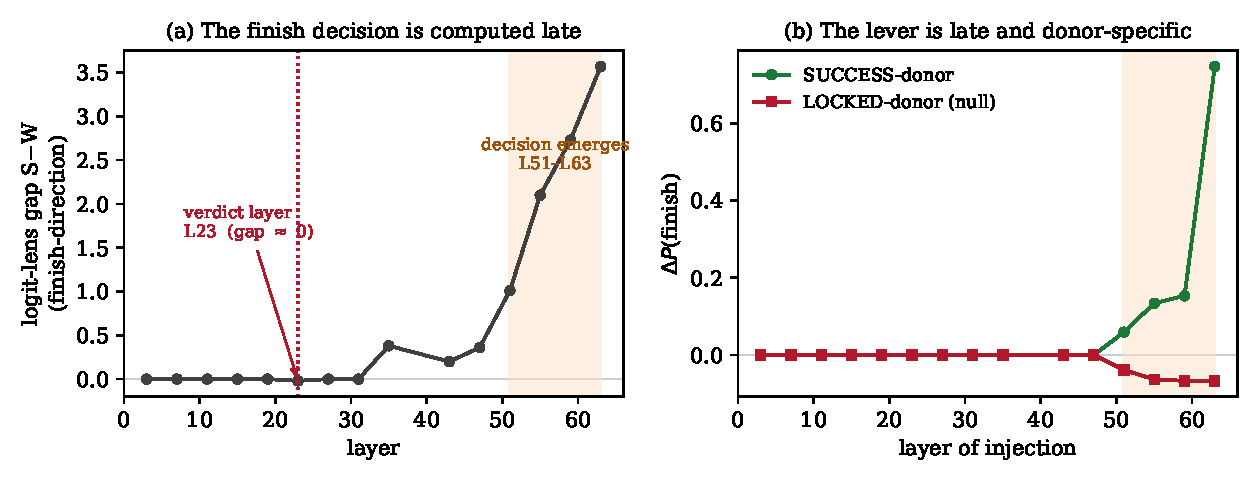
\includegraphics[width=\textwidth]{figures/fig1_layer_sweep.pdf}
\caption{\textbf{The lever is late.} (a) Logit-lens \textsc{success}$-$\textsc{wandering} gap in the \texttt{finish}-direction across layers; flat through L31 (and $\approx 0$ at the verdict layer L23), exploding only in the late block L51--L63 (shaded). Early layers, reported as flat in the run, are drawn at $0$. (b) Activation patching: injecting the \textsc{success} late-block state into \textsc{wandering} raises P(\texttt{finish}) (green) while the \textsc{locked}-donor null (red) moves it the other way; mid/verdict layers are inert. The decision is computed $\sim$30 layers downstream of the verdict.}
\label{fig:sweep}
\end{figure}

\begin{table}[h]
\centering
\caption{Activation patching at the decision point ($n=12$ \textsc{wandering}). $\Delta P(\texttt{finish})$ from injecting each class-donor late-block state; the \textsc{success} donor is the lever, the \textsc{locked} donor the directional null. Mid/verdict layers (L3--L47) are inert.}
\label{tab:patch}
\begin{tabular}{lcccc}
\toprule
donor & L51 & L55 & L59 & L63 \\
\midrule
\textsc{success} (lever) & $+0.059$ & $+0.134$ & $+0.153$ & $+0.747$ \\
\textsc{locked} (null)   & $-0.039$ & $-0.063$ & $-0.067$ & $-0.067$ \\
\bottomrule
\end{tabular}
\end{table}

\subsection{The lever produces a real \texttt{finish} --- but only task-matched}
The one-token probability bump survives a real generation (Table~\ref{tab:gen}, Figure~\ref{fig:gen}). Patching the late-block donor at the decision point and decoding freely makes the agent emit a coherent \texttt{<function=finish>} call (e.g.\ \texttt{=finish> <parameter=output> The issue \dots}), \emph{not} degenerate text. Counting a flip if the agent finishes at any late layer (L55/L59/L63), the \emph{per-pair task-matched} donor flips $5/12$ ($42\%$; exact one-sided McNemar $p=0.031$ versus the $0/12$ baseline), the held-out split reproduces it, and the \textsc{locked} null flips $0/12$. The coarse \textsc{success}-class-mean donor flips only $3/12$ ($25\%$, $p=0.125$, not significant). \textbf{The lever is task-specific}: it requires the matching task's finish-context; a generic class mean washes it out. This is precisely why paper~\#2's generic-direction residual injections were nulls \cite{residual_nulls} --- the right direction is task-conditioned.

\begin{table}[h]
\centering
\caption{Generation confirmation ($n=12$ \textsc{wandering}; finish-emission rate). The any-late-layer union is the headline; $p$ is an exact one-sided McNemar test versus the $0/12$ baseline.}
\label{tab:gen}
\begin{tabular}{lcccc}
\toprule
donor & L55 & L59 & L63 & any-late (union), $p$ \\
\midrule
baseline (no patch) & $0.00$ & $0.00$ & $0.00$ & $0/12$, --- \\
\textsc{locked} (null) & $0.00$ & $0.00$ & $0.00$ & $0/12$, $p=1.0$ \\
\textsc{success}-mean (coarse) & $0.08$ & $0.08$ & $0.17$ & $3/12=0.25$, $p=0.125$ \\
\textsc{success} held-out (split B) & $0.08$ & $0.00$ & $0.17$ & --- \\
\textbf{per-pair (task-matched)} & $\mathbf{0.25}$ & $\mathbf{0.33}$ & $0.17$ & $\mathbf{5/12=0.42}$, $\mathbf{p=0.031}$ \\
\bottomrule
\end{tabular}
\end{table}

\begin{figure}[h]
\centering
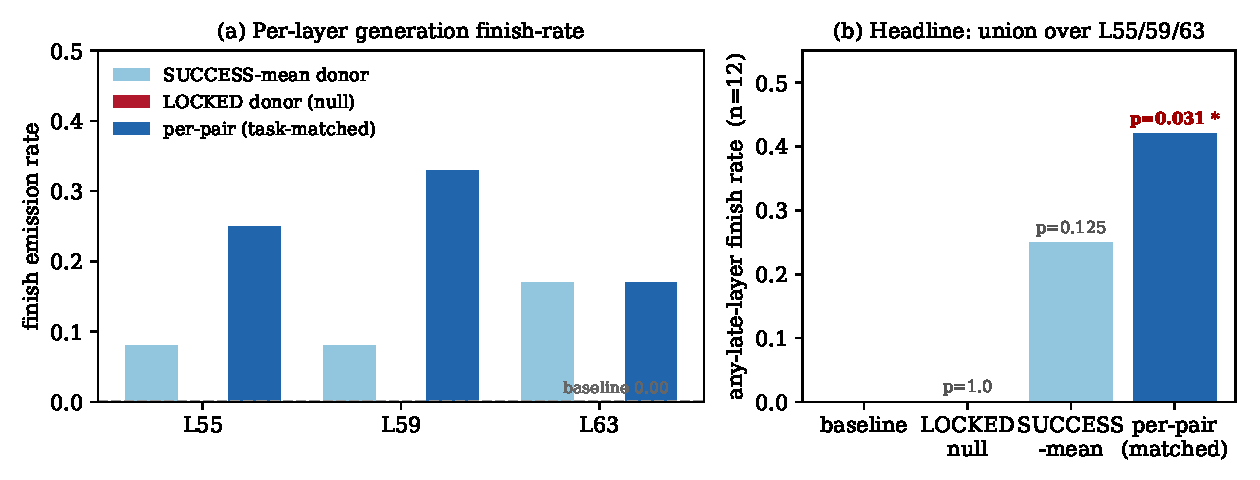
\includegraphics[width=\textwidth]{figures/fig2_generation.pdf}
\caption{\textbf{The lever emits a real \texttt{finish}, and it is task-specific.} (a) Per-layer generation finish-rate; the per-pair task-matched donor (blue) dominates the coarse mean (light) and the \textsc{locked} null (zero). (b) Headline union over L55/L59/L63: the task-matched donor flips $42\%$ of \textsc{wandering} ($p=0.031$) from a $0\%$ baseline, while the coarse mean ($25\%$) is not significant.}
\label{fig:gen}
\end{figure}

\subsection{The law: control is graded by proximity to the action channel}
Reading the arc through this result yields one law (Figure~\ref{fig:law}). Causal control over the termination decision is a graded function of how close the intervention is to the action channel:
\begin{itemize}\itemsep1pt
\item \textbf{verdict feature (L23):} detection only (AUROC $0.91$) --- causal effect $\approx 0$ ($\Delta P = -0.001$) \cite{verdict_circuit};
\item \textbf{late residual block (L55--L63), task-matched:} a partial internal lever --- $42\%$ generation flip, $p=0.031$ (this work);
\item \textbf{action / token channel (behavioral interruption):} the dominant lever --- $30\%\to70\%$ rescue \cite{modality}.
\end{itemize}
Knowledge is consolidated $\sim$30 layers before the action is committed; the late internal state is a genuine but partial lever; the action channel dominates. The gap closes in exactly one place --- late, task-matched, near the action.

\begin{figure}[h]
\centering
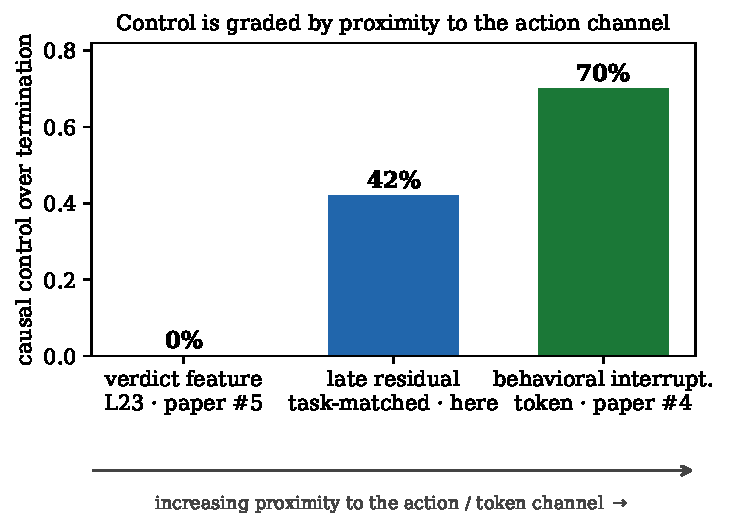
\includegraphics[width=0.62\textwidth]{figures/fig3_graded_law.pdf}
\caption{\textbf{The graded law.} Causal control over termination rises with proximity to the action channel: null at the verdict feature (paper~\#5), partial at the late task-matched residual (this work), dominant at the behavioral/token channel (paper~\#4). The three values come from three arc experiments with different baselines and $n$; the \emph{ordering}, not the exact heights, is the claim.}
\label{fig:law}
\end{figure}

\section{Discussion}\label{sec:discussion}

\textbf{The knowledge--action gap is a layer gap.} The gap of \cite{basu_kag} and the predict/control discrepancy of \cite{bhalla_pc} are, in this agent, spatial: the knowledge (the verdict) is consolidated mid-stream, and the action is committed $\sim$30 layers later. Interventions that read out from or write to the knowledge locus fail because they are in the wrong place; the one that works writes to the late commitment block. This reframes ``detection $\neq$ control'' for agents as a statement about \emph{where} in the network a decision is writable, not \emph{whether} it is.

\textbf{Why the prior nulls were nulls.} The task-specificity result resolves the arc's central tension. Paper~\#2's residual injections used a class-generic \textsc{success} direction and failed; here the class-mean donor is also not significant ($25\%$, $p=0.125$), while the \emph{task-matched} donor is ($42\%$, $p=0.031$). The lever is real but conditioned on the task --- a generic ``finish'' direction does not exist in this agent, which is exactly why every generic intervention in the arc read as a null. This is a constructive explanation of five negative results, not a contradiction of them.

\textbf{The action channel still dominates.} The internal lever is partial ($42\%$) and weaker than the behavioral interruption ($70\%$, \cite{modality}). For practitioners, the ordering is the operational message: the cheapest and strongest control surface for a wandering agent remains behavioral (interrupt and re-prompt), the internal late-block lever is a real but harder-to-wield second option, and the verdict representation is not a control surface at all. ``Read the activations and nudge the verdict feature'' remains the wrong design; ``steer the late commitment block with a task-matched target'' is a viable but expensive one.

\textbf{What this says about \S13.} The arc's \S13 mechanism --- ``the verdict is consolidated but the edge fails to emit'' --- is now precise: the failure is not a broken readout \emph{from} the verdict (restoring the verdict feature does nothing), but a late action-commitment computation that, in \textsc{wandering}, does not reach the \texttt{finish} state. Supplying that late state, task-matched, is what flips it.

\section{The decision locator (released tool)}\label{sec:tool}
The experiment generalizes to a reusable primitive. We release \texttt{decision-locator}, a small, dependency-light, model-agnostic tool that, given any open-weight causal LM and a decision-point prompt, (i) \emph{locates} the layer where a tool/action decision becomes readable (the layer-resolved logit-lens), (ii) \emph{sweeps} activation patching to find the layer where a donor state causally moves the decision, and (iii) \emph{steers} a real generation by patching that layer at the decision position. It is the artifact form of this paper's method: a ``finish-decision locator and late-block steerer'' that runs on any HuggingFace decoder model, with a CPU smoke test on a small model and the Qwen3.6-27B usage documented. Code: \texttt{github.com/OpenInterpretability/openinterp-swebench-harness} under \texttt{tools/decision\_locator/}.

\section{Scope and honest caveats}\label{sec:scope}
Single model (Qwen3.6-27B), single task family (SWE-bench Pro), $n=12$ per class. The headline $p=0.031$ is an exact one-sided McNemar test with all five discordant pairs flipping one way against a definitional $0/12$ baseline; the per-layer rates are noisy at this $n$ (e.g.\ the held-out split flips $0/12$ at L59 while the task-matched donor flips $4/12$). \emph{The coarse-mean donor is not significant} ($p=0.125$) --- the positive claim depends on the task-matched donor. The effect is partial ($42\%$) and weaker than the behavioral channel. L63's large patching $\Delta P$ ($+0.747$) is near the output and partly trivial; the load-bearing patching evidence is L51--L59 ($+0.06$ to $+0.15$). The graded law (Figure~\ref{fig:law}) synthesizes three experiments with different baselines and $n$ --- the ordering is the claim, not a single controlled measurement. Generation is greedy; prompts are truncated to $4000$ tokens (the fidelity gate confirms the decision state survives). We claim: a task-matched late-block state, patched at the decision point, causally produces a real \texttt{finish} in a significant fraction of \textsc{wandering} runs --- the first internal causal lever of the arc --- and the broader law that control is graded by proximity to the action channel.

\section{Conclusion}\label{sec:conclusion}
After five papers locating where control over a long-horizon agent's termination is \emph{not} --- not the residual, not the right locus, not the named verdict feature --- this paper locates where it \emph{is}: a late, task-matched action-commitment block, $\sim$30 layers downstream of the verdict, where a patched \textsc{success} state makes a \textsc{wandering} agent emit a real \texttt{finish} in $42\%$ of cases ($p=0.031$). The knowledge--action gap on agents is a layer gap, and it closes near the action channel. The arc's five nulls were not evidence of an unsteerable agent; they were the map that pointed to the one place the lever lives.

\paragraph{Data and code availability.} This is the first positive of the WANDERING arc \cite{tool_entropy,residual_nulls,multichannel,modality,verdict_circuit,companion_note}. All artifacts are public:
\begin{itemize}\itemsep1pt
\item Code (pre-registration, figure code, breakthrough and confirmation notebooks, per-experiment results, and the released tool): the arc repository \texttt{OpenInterpretability/openinterp-swebench-harness} on GitHub, under \texttt{paper/breakthrough/}, \texttt{notebooks/}, and \texttt{tools/decision\_locator/}.
\item Data (trajectory transcripts, labels, residual bundle): the HuggingFace dataset \texttt{caiovicentino1/swebench-phase6-verdict-circuit}.
\item SAE: \texttt{caiovicentino1/qwen36-27b-sae-fullstack}.
\end{itemize}

\begin{thebibliography}{99}
\bibitem{tool_entropy} C. Vicentino. Tool-Entropy Collapse: A Cross-Architecture Signature of Agent WANDERING Failure. Zenodo, 2026. DOI 10.5281/zenodo.20368601.
\bibitem{residual_nulls} C. Vicentino. Causal Localization of Agent WANDERING to Edge-Layer L11: The Right Locus Is Still Not a Rescue Lever. Zenodo, 2026. DOI 10.5281/zenodo.20490278.
\bibitem{multichannel} C. Vicentino. Multi-Channel Mechanistic Signatures of Agent WANDERING: Classification, Causal Localization, and Behavior-Legible Response to Intervention. Zenodo, 2026. DOI 10.5281/zenodo.20490284.
\bibitem{modality} C. Vicentino. Modality Matters: A Transient Behavioral Interruption Rescues Agent WANDERING Where Residual Steering Does Not. Zenodo, 2026. DOI 10.5281/zenodo.20490286.
\bibitem{verdict_circuit} C. Vicentino. The Verdict Is Not the Lever: An Interpretable Task-Completion Feature Predicts but Does Not Cause Long-Horizon Agent Termination. Zenodo, 2026. DOI 10.5281/zenodo.20532769.
\bibitem{companion_note} C. Vicentino. No Better Than Behavioral: A Residual Velocity-Freezing Fingerprint Predicts Agent WANDERING No Better Than the Cheap Tool-Entropy Detector. Zenodo, 2026. DOI 10.5281/zenodo.20500053.
\bibitem{basu_kag} Basu et al. Interpretability without actionability: mechanistic methods cannot correct language model errors despite near-perfect internal representations. arXiv:2603.18353, 2026.
\bibitem{bhalla_pc} Bhalla et al. Towards Unifying Interpretability and Control: Evaluation via Intervention. arXiv:2411.04430, 2024.
\end{thebibliography}

\end{document}
